\documentclass[t,xcolor={usenames,dvipsnames}]{beamer}

\mode<presentation>
{
\usetheme{Frankfurt}%{Warsaw}
%\setbeamercovered{transparent}
%\setbeamercolor{background canvas}{bg=white}
}

% Delete these, if you do not want the table of contents to pop up at
% the beginning of each (sub)section:
%\AtBeginSubsection[]
%{
%  \begin{frame}<beamer>{Outline}
%    \tableofcontents[currentsection,currentsubsection]
%  \end{frame}
%}
%\AtBeginSection[]
%{
%  \begin{frame}<beamer>{Outline}
%    \tableofcontents[currentsection]
%  \end{frame}
%}

\usepackage[english]{babel}
\usepackage[latin1]{inputenc}
\usepackage{times}
\usepackage[T1]{fontenc}
\usepackage{verbatim}
\usepackage{url}
\usepackage{amsmath,amssymb}
\usepackage{comment}
\usepackage[overlay,absolute]{textpos}
\usepackage{hyperref}

% Author-date citations
\usepackage[authoryear,round]{natbib}
\let\cite=\citep  % default \cite such as {\LaTeX} authors are used to

% Where \includegraphics should look for figures
\graphicspath{{./figs/}}
\usepackage{epstopdf}
\DeclareGraphicsExtensions{.eps,.png,.jpg,.pdf}

% Shortcuts
\newcommand{\myhref}[2]{\href{#1}{\textcolor{Blue}{#2}}}
\newcommand{\myurl}[1]{\myhref{#1}{#1}}
\newcommand{\subitem}[1]{\begin{itemize}[<.->]\item #1 \end{itemize}}
\newcommand{\ghead}[1]{{\tiny #1\\}}
\newcommand{\doi}[1]{\myhref{http://dx.doi.org/#1}{doi:#1}}
\newcommand{\csym}[1]{\textcolor{Blue}{\texttt{#1}}}
\newcommand{\ud}{\mathrm{d}}
\newcommand{\dt}{\ud t}

%%%%%%%%%%%%%%%%%%%%%%%%%%%%%%%%%%%%%%%%%%%%%%%%%%%%%%%%%%%%%%%%%%%%%%
\title{Further Adventures in Functional Curation}
\author{Jonathan Cooper}
\institute[University of Oxford]
{Computational Biology Group\\
 Department of Computer Science\\
 University of Oxford}
\date{January 30, 2013}

\begin{document}

%%%%%%%%%%%%%%%%%%%%%%%%%%%%%%%%%%%%%%%%%%%%%%%%%%%%%%%%%%%%%%%%%%%%%%

%%%%%%%%%%%%%%%%%%%%%%%%%%%%%%%%%%%%%%%%%%%%%%%%%%%%%%%%%%%%%%%%%%%%%%
\section{Introduction to functional curation}
\subsection*{Main}
%%%%%%%%%%%%%%%%%%%%%%%%%%%%%%%%%%%%%%%%%%%%%%%%%%%%%%%%%%%%%%%%%%%%%%

\begin{frame}{Motivation}
\begin{itemize}
\item Want ONE copy of my model (defined in ONE CellML file)
\item Want to do a number of different complicated interventions, e.g.\ changing pacing rate (fairly easy in Chaste)
\item Our FC system allows you to extend this to any model modifications
  \begin{itemize}
  \item e.g.\ clamp some concentrations (remove $\frac{\ud u}{\dt}$, set $u$ constant)
  \item Previously had to modify generated C++ or CellML manually
  \item Better to define modifications in one place, so can apply to any model at any time
  \end{itemize}
\item (And it runs the simulation, performs post-processing and plots graphs for you too!)
\item ``In fact it does sound rather good'' - Gary Mirams
\end{itemize}
\end{frame}


\begin{frame}{Setting the context}
\begin{itemize}
\item Many models are available in languages such as CellML
\item But, how can we\ldots
  \begin{itemize}
  \item Determine a model's functionality, i.e.\ its suitability or limitations for a new study?
  \item Re-use a model in a different experimental context?
  \item Compare different models' behaviours under the same experiment?  (Compare hypotheses.)
  \end{itemize}
\end{itemize}
\end{frame}


\begin{frame}{Goal of this work}
\begin{itemize}
\item Provide a framework for a coherent approach to model fitting, simulation, comparison and validation
  \begin{itemize}
  \item Continuous evaluation of model predictions against experimental data, throughout model lifecycle
  \item Models that are robust, well tested, and well characterised for particular biological studies
  \item Model development akin to high quality software
  \end{itemize}
\end{itemize}
\end{frame}


\begin{frame}{How do we get there?}
\subitem{Separate \alert{model structure} and \alert{experimental scenario}}
\begin{center}
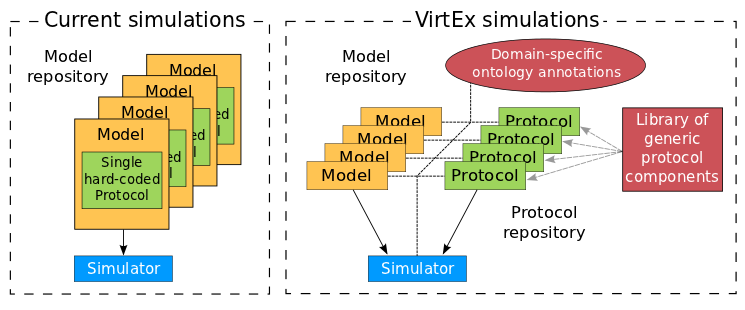
\includegraphics[width=.9\textwidth]{VirtEx_overview}
\end{center}
\end{frame}


%%%%%%%%%%%%%%%%%%%%%%%%%%%%%%%%%%%%%%%%%%%%%%%%%%%%%%%%%%%%%%%%%%%%%%
\begin{frame}{Acknowledgments}
Gary Mirams\\
Chaste team\\
Alan Garny, Steven Niederer, David Gavaghan

Reference publication: \doi{10.1016/j.pbiomolbio.2011.06.003}\\
Website: \myurl{https://chaste.cs.ox.ac.uk/trac/wiki/FunctionalCuration}

\begin{center}

\includegraphics[scale=.9]{chaste-266x60}\\ \vspace{.3cm}

\includegraphics[scale=.7]{logo2020science}\\ \vspace{.4cm}

\includegraphics[width=.55\textwidth]{EPSRC1RGBLO} \hspace{.1cm}

\includegraphics[scale=.55]{logo_msr}
\end{center}
\end{frame}


%%%%%%%%%%%%%%%%%%%%%%%%%%%%%%%%%%%%%%%%%%%%%%%%%%%%%%%%%%%%%%%%%%%%%%
\appendix



\end{document}
